\subsection{Radar depth and error}
In addition to constraining the age of englacial reflectors with the Byrd ice core chronology, we also quantify uncertainty in their radar-observed depth, another source of error in the age-depth profile. The ice-penetrating radar used in this analysis was collected in several surveys conducted by the University of Texas Institute for Geophysics, including GIMBLE \citep{young2012}, CASERTZ \citep{morse2002}, and SOAR/WMB \citep{luyendyk2003}. Data has been collected from a DC-3 or Twin Otter airborne platform and uses the HiCARS radar system with 60 MHz center frequency and 15 MHz bandwidth \citep{peters2005}. Radar pulses transmitted into the ice sheet reflect off surfaces of dielectric contrast in the ice which are the result of variations in ice fabric, composition, temperature, rheology, etc \citep{fujita2000}. The reflected signal is received by the radar system and recorded as two-way travel time (TWTT) from transmission to receipt. 


\begin{figure}[h]\label{fig:radarmap}
\centering
\makebox[\textwidth][c]{\includegraphics[scale=0.5]{../analysis/figures/WAISall_bedmap2_final}}
%\captionsetup{width=.9\textwidth}
\caption{Map of central West Antarctic with available airborne geophysical radar surveys (black lines) and (\textbf{will be updated to have:} WAIS Divide and Byrd ice core locations (blue triangles) overlain. Gray shading is surface elevation \citep{fretwell2013}. }

\end{figure}



In this study, we consider TWTT of four reflectors spanning the ice thickness in the region of central West Antarctica (Figure~\ref{fig:layergram}). These reflectors have been tracked extensively using Halliburton's Landmark seismic interpretation software and can be tied to both the Byrd and WAIS Divide ice cores for dating. %Determining the depth of the reflectors, $D_r$, may be affected by several sources of uncertainty, including uncertainty in the firn depth, the velocity of the radar pulse in ice, and the pulse-limited precision of radar observations.

\begin{figure}[h]
\centering
\makebox[\textwidth][c]{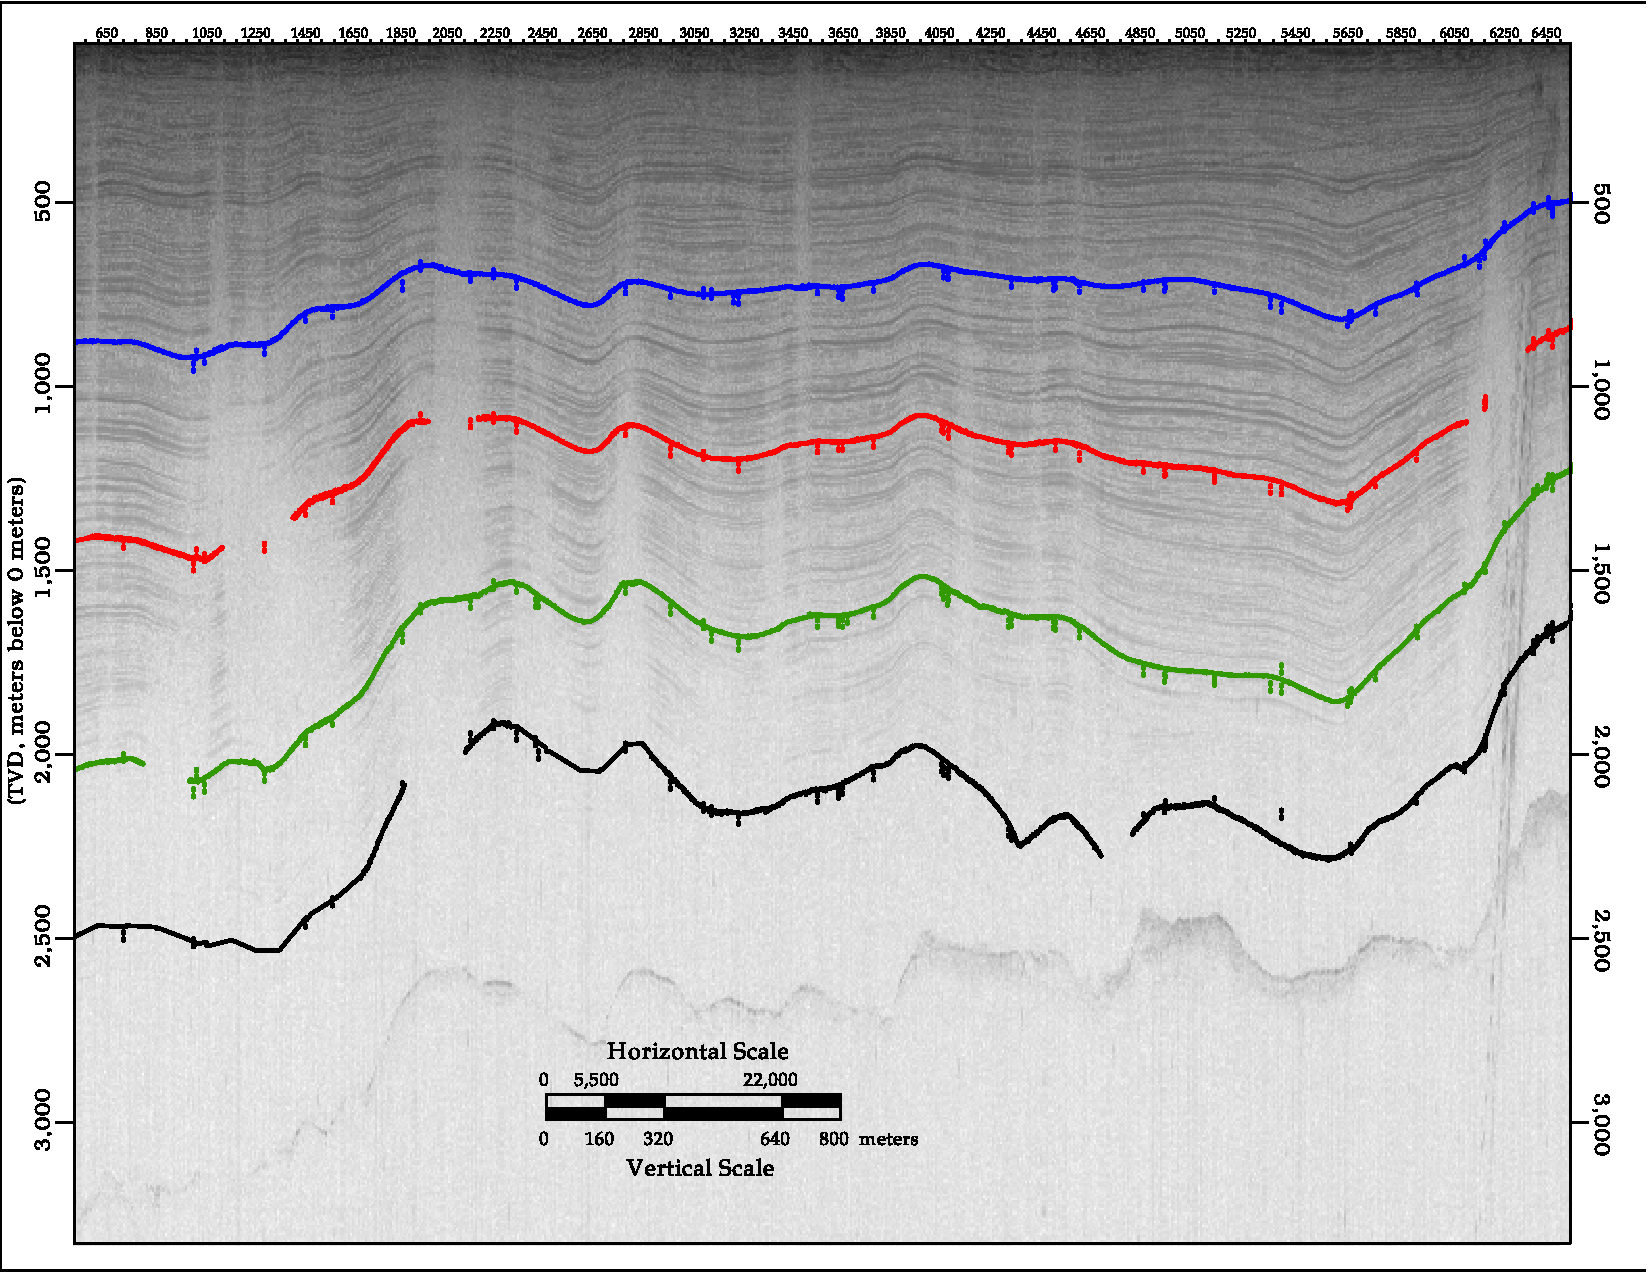
\includegraphics[scale=0.6]{figures/radargram-4layers-paper}}
%\captionsetup{width=.9\textwidth}
\caption{Radargram showing reflectors of interest near the Byrd ice core.  }
\label{fig:layergram}
\end{figure}


To estimate reflector depths, $D_r$, we begin with a simple relation assuming known velocity of the signal in air and in ice (first term in Equation \ref{deptheqn}). We also incorporate several known sources of uncertainty, including: 1) variations in the signal velocity in ice due to ice temperature and fabric, 2) vertical resolution limitations resulting from digitized pulse width sampling effects, and 3) measurement errors in the density profile needed to account for the changing signal velocity in the firn (Equation \ref{deptheqn}).

\begin{equation}\label{deptheqn}
D_i = \frac{1}{2}~TWTT \cdot \vec{v} + \epsilon_{v_{ice}} + \epsilon_{PW} + \epsilon_{firn}
\end{equation}

The first source of error, $\epsilon_{v_{ice}}$, results from ice temperature, crystal structure, anisotropy, and other ice fabric effects. EM velocity in ice, $v_{ice}$, varies from 168 to 169.5 $m/{\mu}s$ \citep{fujita2000} and the integration of these errors leads to increasing uncertainty with depth.  The complexity of local ice properties affecting the velocity at any location and depth make it difficult to know the error distribution, so we make the simplifying assumption that this error is uniform. Constant values of $v_{ice}$ are therefore sampled from a uniform distribution: $p(v_{ice}) ~\sim U(168~m/{\mu}s,169.5~m/{\mu}s)$.

The radar pulse width determines its vertical resolution \citep{millar1982}. We assume a finite pulse width, meaning that an infinitesimally thin layer of ice will appear in the survey to have a finite width. This can lead to errors in tracing reflectors and identifying their depths. The error in phase sampling of the EM pulse, $\epsilon_{PW}$, is taken to be a function of the wavelength of the pulse, $\lambda$. The sampling rate for the data used here varies from 5 ns to 20 ns. We assume a 10 ns resolution when tracking the phase of layer detections and assume this error is normal.

Finally, in the upper part of the ice sheet, a firn layer of less density than glacial ice acts to slow the velocity of the radar signal. To deal with this, we use a firn correction to accurately estimate the depth to radar reflectors. All englacial reflectors of interest in this study are deeper than the firn layer, so a single firn correction---the difference between the ice thickness with and without the firn layer present---is added to layer depths to correction for the underestimation of depth if the firn layer is not considered. The firn correction, $d_{firn}$, is treated as a model parameter for which we invert. Based on density measurements at the Byrd ice core site \citep{gow1970}, bounds can be placed on the firn layer thickness and therefore the firn correction. We assume the firn correction to be less than the firn layer depth and sample values from a uniform distribution: $p(d_{firn})\sim$ U(1~m, 65~m). %Errors in density, $\rho(z)$, are available for the WAIS Divide measurements. These are assumed gaussian, randomly sampled, and the firn correction is computed using the \citet{dowdeswell2004} relation:

%\begin{equation}
%z_f = \frac{K}{n^{'}_{i}}\int{(\rho_{i} - \rho(z)) dz}
%\end{equation}
%where K is 0.85 m$^{3}$ Mg$^{-1}$ \citep{robin1969}, $n^{'}_{i}$ is the refractive index of ice ($n^{'}_{i}$=1.78), $\rho_{i}$ is the density of ice ($\rho_{i}$=0.917 Mg m$^{-3}$) and $\rho(z)$ is the density of ice at depth \textit{z} with units Mg m$^{-3}$.

We assume constant velocities, $\vec{v}$, in air (300 m/${\mu}$s) and ice. The TWTT from the observing aircraft to the surface of the ice sheet is known from interpretation of the surface reflector and the remainder of the signal is assumed to be in glacial ice. The computed depth of each reflector is relative to the ice surface as also measured by the HiCARS radar. While each layer may have depth errors independent of the others, errors in the distance between the surface and the acquisition aircraft are systematic across all observed reflectors in the ice column. Therefore, a pulse-width error, randomly sampled error, $\epsilon_{PW}$, is also sampled for the ice sheet surface and the same error is applied to all radar reflectors in the column. 







